%----------------------------------------------------------------------------------------
%	PACKAGES AND OTHER DOCUMENT CONFIGURATIONS
%----------------------------------------------------------------------------------------

\documentclass[
12pt, % The default document font size, options: 10pt, 11pt, 12pt
%oneside, % Two side (alternating margins) for binding by default, uncomment to switch to one side
english, % ngerman for German
singlespacing, % Single line spacing, alternatives: onehalfspacing or doublespacing
%draft, % Uncomment to enable draft mode (no pictures, no links, overfull hboxes indicated)
%nolistspacing, % If the document is onehalfspacing or doublespacing, uncomment this to set spacing in lists to single
%liststotoc, % Uncomment to add the list of figures/tables/etc to the table of contents
%toctotoc, % Uncomment to add the main table of contents to the table of contents
%parskip, % Uncomment to add space between paragraphs
%nohyperref, % Uncomment to not load the hyperref package
headsepline, % Uncomment to get a line under the header
%chapterinoneline, % Uncomment to place the chapter title next to the number on one line
%consistentlayout, % Uncomment to change the layout of the declaration, abstract and acknowledgements pages to match the default layout
]{MastersDoctoralThesis} % The class file specifying the document structure

\usepackage[utf8]{inputenc} % Required for inputting international characters 
\usepackage[T1]{fontenc} % Output font encoding for international characters

\usepackage{mathpazo} % Use the Palatino font by default

\usepackage[
	backend=bibtex,
	style=numeric,
	natbib=true
]{biblatex} % Use the bibtex backend with the authoryear citation style (which resembles APA)

\addbibresource{bibliography.bib} % The filename of the bibliography

\usepackage[autostyle=true]{csquotes} % Required to generate language-dependent quotes in the bibliography

%----------------------------------------------------------------------------------------
%	MARGIN SETTINGS
%----------------------------------------------------------------------------------------

\geometry{
	paper=a4paper, % Change to letterpaper for US letter
	inner=3.0cm, % Inner margin
	outer=2.5cm, % Outer margin
	bindingoffset=.5cm, % Binding offset
	top=1.5cm, % Top margin
	bottom=1.5cm, % Bottom margin
	%showframe, % Uncomment to show how the type block is set on the page
}

%----------------------------------------------------------------------------------------
%	THESIS INFORMATION
%----------------------------------------------------------------------------------------

\thesistitle{Clustering aggregation on a neutral atom quantum computer} 
\supervisor{Prof. Stefano Lodi} 
\cosupervisor{Dr. Gabriella Bettonte\\Dr. Antonio Costantini}
\degree{Master's Degree in Computer Science} 
\author{Riccardo Scotti} 


\subject{Computer Science} 
\keywords{} 
\university{\href{http://www.unibo.it/en}{University of Bologna}} 
\department{\href{https://disi.unibo.it/en}{Department of Computer Science and Engineering}} 
\group{\href{http://researchgroup.university.com}{Research Group Name}} 
\faculty{\href{http://www.scienze.unibo.it/en}{School of Science}} 

\AtBeginDocument{
	\hypersetup{
		pdftitle=\ttitle,
		pdfauthor=\authorname,
		pdfkeywords=\keywordnames,
		linkcolor=black,
		urlcolor=black
	}
}

\begin{document}

\frontmatter 

\pagestyle{plain} 

%----------------------------------------------------------------------------------------
%	TITLE PAGE
%----------------------------------------------------------------------------------------


\begin{titlepage}
  \begin{center}
      {{\Large{\textsc{Alma Mater Studiorum $\cdot$ University of Bologna}}}}
      \rule[0.1cm]{\textwidth}{0.1mm}
      \rule[0.5cm]{\textwidth}{0.6mm}\\
      {\small{\bf School of Science\\
      Department of Computer Science and Engineering\\
      Master's Degree in Computer Science}}
  \end{center}
  
  \vspace{25mm}
  
  \begin{center}
      
      {\LARGE{\bf Clustering aggregation on}}\\
      \vspace{3mm}
      {\LARGE{\bf a neutral atom quantum computer}}\\
  \end{center}
  
  \vspace{60mm}
  \par
  \noindent
  \begin{minipage}[t]{0.04\textwidth}
  ~
  \end{minipage}
  \begin{minipage}[t]{0.4\textwidth}
  {\large{\textbf{Supervisor}:\\
  \supname
  }}
  \end{minipage}
  \hfill
  \begin{minipage}[t]{0.4\textwidth}\raggedleft
  {\large{\textbf{Submitted by}:\\
  \authorname}}
  \end{minipage}
  \begin{minipage}[t]{0.04\textwidth}
  ~
  \end{minipage}
  
  \vspace{10mm}
  \begin{minipage}[t]{0.4\textwidth}
  \large{\textbf{Cosupervisors}:\\
  \cosupname}
  \end{minipage}
  
  \vspace{30mm}
  
  \begin{center}
      {\large{\bf Session II\\
      Academic Year 2023/2024 }}
  \end{center}
  \end{titlepage}

%----------------------------------------------------------------------------------------
%	ABSTRACT PAGE
%----------------------------------------------------------------------------------------

\begin{abstract}
\addchaptertocentry{\abstractname} % Add the abstract to the table of contents
TODO
\end{abstract}

%----------------------------------------------------------------------------------------
%	ACKNOWLEDGEMENTS
%----------------------------------------------------------------------------------------

\begin{acknowledgements}
\addchaptertocentry{\acknowledgementname} % Add the acknowledgements to the table of contents
TODO
\end{acknowledgements}

%----------------------------------------------------------------------------------------
%	ABBREVIATIONS
%----------------------------------------------------------------------------------------

% \begin{abbreviations}{ll} % Include a list of abbreviations (a table of two columns)

% \textbf{LAH} & \textbf{L}ist \textbf{A}bbreviations \textbf{H}ere\\
% \textbf{WSF} & \textbf{W}hat (it) \textbf{S}tands \textbf{F}or\\

% \end{abbreviations}

%----------------------------------------------------------------------------------------
% TABLE OF CONTENTS
%----------------------------------------------------------------------------------------

\tableofcontents % Prints the main table of contents

%----------------------------------------------------------------------------------------
%	THESIS CONTENT - CHAPTERS
%----------------------------------------------------------------------------------------

\mainmatter % Begin numeric (1,2,3...) page numbering

\pagestyle{thesis} % Return the page headers back to the "thesis" style

% Include the chapters of the thesis as separate files from the Chapters folder
% Uncomment the lines as you write the chapters

\chapter{Introduction}
TODO
\chapter{Background}
\label{cha:background}

\section{Clustering}
Clustering is an unsupervised data analysis technique that can be informally defined as the partitioning of a set of objects into groups called clusters; such partitioning must ensure that objects within a same cluster are more similar\footnote{Provided that a binary ordering relation is defined on the set of objects.} to each other than to objects in other clusters. \cite{clustering}

Clustering is widely employed in numerous scenarios that require to group together similar data points, or to extract knowledge from a set of objects in the absence of any prior information. For instance, it is used in marketing and finance as a profiling tool; % ref: TODO
in image processing and computer vision, as a segmentation technique \cite{Gonzalez2017}, where it plays a pivotal role in various fields, such as remote image sensing \cite{remote-sensing} and digital forensics \cite{forensics}; % ref: gonzalez image processing capitolo su segmentation
by energy distribution companies, to optimize the allocation of resources to end users. % ref: TODO

\subsection{Formal definition}
Let $D = \{x_{1},...,x_{n}\}$ be a set of objects, also called \textit{dataset}; a clustering for $D$ is a collection of $k$ elements $\mathcal{C} =\{c_{1},...,c_{k}\}$, with $\mathcal{C} \subseteq \mathcal{P}(D)$, such that the following properties hold:
\begin{equation}
    \label{eqn:union}
    D = \bigcup_{i=1}^{k} c_{i}
\end{equation}
\begin{equation}
    \label{eqn:overlap}
    c_{i} \cap c_{j} = \emptyset \quad \forall c_{i}, c_{j} \in \mathcal{C}.
\end{equation}

\subsection{Clustering aggregation}


\section{Quantum computing}
Quantum computing is a set of computational models and paradigms that combine concepts of computer science, physics and engineering. It offers an theoretical framework alternative to that of classical computing, which proved to be beneficial in certain areas of interest, such as cryptography and optimization. % ref?

The basic ideas of quantum computing were established by Richard Feynman in a 1982 paper, discussing the usage of computers to perform physics simulations \cite{Feynman1982}. Feynman observed that, due to their inherent complexity, quantum systems could not be feasibly simulated by classical computers, and introduced the idea of computing machines based on quantum principles \cite{Feynman2017}. A subsequent work by Deutsch demonstrated, via the construction of a quantum Turing machine, that quantum computers are computationally equivalent to classical computers, and could therefore be useful for scopes beyond mere quantum simulation \cite{deutsch1985quantum}.

\subsection{Elements of quantum computing}
% citare Nielsen-Chuang
The fundamental unit of information in quantum computing is the quantum bit, or qubit for short. Regardless of their physical realization, qubits are characterized by their state, which carries information. While the state of a classical bit is always only one of two logical values (usually called \texttt{0} and \texttt{1}), the state of a qubit works in a significantly different manner, reflecting the underlying principles of quantum mechanics. 

% aggiungere postulati di QM? (Kaye-Laflamme-Mosca)
Similarly to its classical counterpart, when the state of a qubit $\ket{\psi}$ is measured, it can assume either one of two logical values (usually called $\ket{0}$ and $\ket{1}$); the key difference with a bit is that the state of a qubit before it is measured is a linear combination of the two possible states:
\begin{equation}
  \ket{\psi} = \alpha \ket{0} + \beta \ket{1},
\end{equation}
where $(\alpha, \beta)$ is a unit vector of a Hilbert space or, in other words, $|\alpha|^{2} + |\beta|^{2} = 1$.

\section{Quantum annealing}

\section{Neutral atoms technology}
\chapter{State of the art}
% stato dell'arte: principalmente quantum, vantaggi portati in alcune applicazioni (ottimizzazione)
	% cfr tesi di dottorato di gabriella 
	% chiedere a lodi per clustering 
\chapter{Proposed method}
\chapter{Experimental setup}
This chapter provides a description of the experimental setup used to evaluate the clustering aggregation protocol in different quantum computing environments, both on a simulator and on real hardware. The protocol was tested on three distinct platforms: a simulator for a neutral-atom quantum computer, specifically the Pulser simulator by PASQAL; the Fresnel neutral-atom quantum computer, also developed by PASQAL; the Advantage quantum annealer with Pegasus topology, developed by D-Wave.

% aggiungere descrizione macchine 
\section{Quantum platforms}
\subsection{Programmable neutral-atom arrays}

\subsection{QuTiP}
The Quantum Toolbox in Python, also known as QuTiP, is an object oriented Python framework designed to represent and simulate the dynamics of open and closed quantum systems \cite{Johansson2012}. 

The core of information representation in QuTiP is the \texttt{Qobj} class, which is used to represent both quantum states (such as pure states or density matrices) and quantum operators (such as Hamiltonians or measurement operators). The \texttt{Qobj} class offers methods to perform matrix operations like addition, multiplication and tensor product, which are essential to manipulate quantum systems; sparse matrix encoding of objects allows these operations to be executed relatively efficiently.

To perform simulations using QuTiP, it is necessary to specify the initial conditions of the system, for example ket vectors or density matrices, and a Hamiltonian or other operators, which describe the time evolution and possible dissipations. It is then possible to select different kinds of solvers, such as the Monte Carlo wave function method for a Schrödinger equation describing evolution of pure states, or a numerical approach for a Lindblad master equation in the case of open systems.

Results are presented in the form of evolved states at fixed intervals throughout the simulation time windows. Additionally, QuTiP allows to perform the calculations of expectation values for observables (such as spin, position, or energy) over time.

Since QuTiP does not directly support neutral-atom systems, Pulser contains a library that acts as an interface to QuTiP, in order to simplify the definition of neutral-atom arrays and the simulation of experiments with laser pulses. 

\section{Dataset}
\label{sec:dataset}
The dataset used to test the protocol is shown in figure \ref{fig:dataset}. It was first introduced by Gionis, Mannila and Tsaparas to test classical clustering aggregation algorithms \cite{dataset}; it was then used by Li and Latecki to test a clustering aggregation protocol that uses simulated annealing \cite{aggregation}.

It is specifically designed to contain different shapes and configuration of points, in such a way that most clustering algorithms fail to produce a correct clustering. It is made up of 7 clusters and 788 points in total.

\begin{figure}[ht!]
  \centering 
  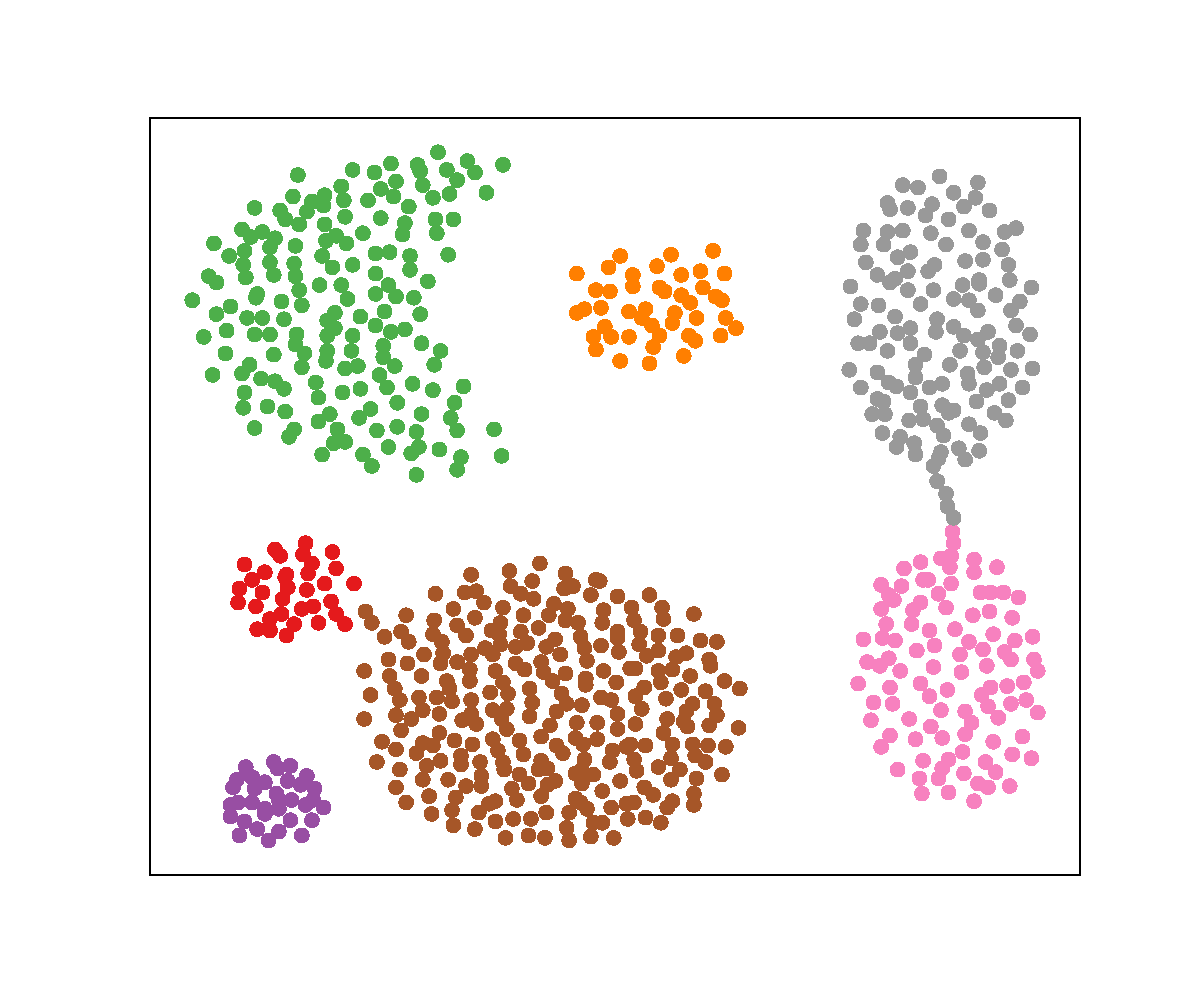
\includegraphics[width=0.72\textwidth]{figures/05experimental_setup/dataset.pdf}
  \caption{Dataset plot}
  \label{fig:dataset}
\end{figure}

\section{Evaluation metrics}
Different metrics were used to evaluate the quality of single clusters and of clustering algorithms as a whole. Silhouette score was used as a factor to weigh clusters in the clustering aggregation protocol; Rand index was used to compare the overall quality of the clustering algorithms and aggregation protocols. % aggiungere anche intersezione insiemistica? 

\subsection{Silhouette score}
The silhouette score is a metric used to evaluate clustering quality, introduced by Rousseeuw \cite{Rousseeuw1987}. The score is computed for each point in the dataset and reflects both its cohesion with points in the same cluster, as well as the separation with respect to points in different clusters. Specifically, the silhouette score of a point $p$ in the dataset is defined as 
\begin{equation}
  \label{eqn:silhouette}
  S_{p} = \frac{b_{p} - a_{p}}{\max({a_{p}, b_{p}})},
\end{equation}
where $a_{i}$ is the average distance from the point to other points in the same cluster (intra-cluster distance), and $b_{i}$ is the average distance to points in the nearest different cluster (inter-cluster distance). The score ranges between -1 and 1, where values close to 1 indicate that points are well-clustered, with high cohesion and good separation, while negative values suggest points may have been assigned to the wrong cluster. 

A quantification of the quality for a single cluster can be obtained by computing the average of the silhouette score of the point it contains; more formally, for a cluster $c_{i}$, the formula for its average silhouette ($AS_{i}$) is 
\begin{equation}
  \label{eqn:cluster_silhouette}
  AS_{i} = \frac{\sum_{p \in c_{i}} S_{p}}{|c_{i}|}.
\end{equation}

\subsection{Rand index}
The Rand index is a metric that quantifies the similarity between two data clusterings, first proposed by Rand \cite{Rand1971}. It is computed by considering all possible pairs of points in the dataset and assessing whether they are assigned to the same or different clusters in the two clusterings being compared. The index assumes values between 0 and 1, with 1 indicating perfect agreement between the two clusterings. 

Given two clusterings $\mathcal{C}_{1}$ and $\mathcal{C}_{2}$, their Rand index is computed as  
\begin{equation}
  \label{eqn:rand}
  RI = \frac{a + b}{a + b + c + d},
\end{equation}
where
\begin{itemize}
  \item $a$ is the number of point pairs that are put in the same cluster in both clusterings;
  \item $b$ is the number of point pairs that are put in different clusters in both clusterings; 
  \item $c$ is the number of point pairs that are put in the same cluster in $\mathcal{C}_{1}$, but in different clusters in $\mathcal{C}_{2}$;
  \item $d$ is the number of point pairs that are put in different clusters in $\mathcal{C}_{1}$, but in the same cluster in $\mathcal{C}_{2}$.
\end{itemize}

\section{Description of experiments}

\subsection{Pulser experiment}
The Pulser neutral-atom computer simulator was used to test the aggregation protocol on the dataset discussed in \ref{sec:dataset}; 

Two different clustering algorithms were run on the dataset, DBSCAN and Spectral Clustering. Hyperparameters were tuned empirically, in order to ensure an overall amount of clusters inferior or equal to 14, so as not to exceed the amount of qubits the simulator can handle \cite{Johansson2012}.

\begin{figure}
  \centering 
  
\end{figure}
\chapter{Results}

\section{Fresnel experiment}

\begin{figure}[ht!]
  \centering
  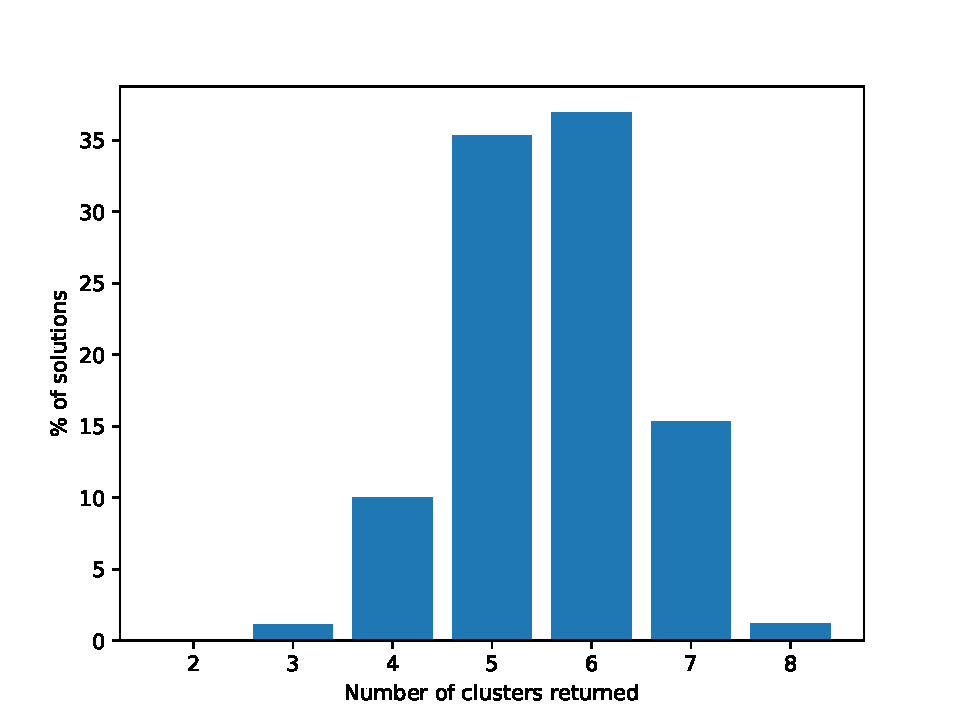
\includegraphics[width=0.6\textwidth]{figures/06results/num_clusters.pdf}
  \caption{Histogram for probability of number of clusters returned in Fresnel experiment}
\end{figure}

\begin{table}[ht]
  \centering
  \begin{tabular}{|c|c|}
      \hline
      Number of clusters & Probability (\%) \\
      \hline
      2 & 0.12 \\ 
      3 & 1.11 \\ 
      4 & 10.0 \\ 
      5 & 35.31 \\ 
      6 & 36.91 \\ 
      7 & 15.31 \\ 
      8 & 1.23 \\ 
      \hline
  \end{tabular}
  \caption{Probability of number of clusters returned in Fresnel experiment}
\end{table}
\chapter{Conclusions}

%----------------------------------------------------------------------------------------
%	THESIS CONTENT - APPENDICES
%----------------------------------------------------------------------------------------

\appendix % Cue to tell LaTeX that the following "chapters" are Appendices

% Include the appendices of the thesis as separate files from the Appendices folder
% Uncomment the lines as you write the Appendices

% \include{Appendices/AppendixA}
% \include{Appendices/AppendixB}
% \include{Appendices/AppendixC}

%----------------------------------------------------------------------------------------
%	LIST OF FIGURES/TABLES PAGES
%----------------------------------------------------------------------------------------

\listoffigures % Prints the list of figures

\listoftables % Prints the list of tables

%----------------------------------------------------------------------------------------
%	BIBLIOGRAPHY
%----------------------------------------------------------------------------------------

\printbibliography[heading=bibintoc]

%----------------------------------------------------------------------------------------

\end{document}  